\section{Experiments and Results}

\begin{table}
  \begin{center}
  \begin{tabular}{|l||r|}
    \hline
    & VBS Delta Encoding \\ \hline
    Volcano & 53.3\% \\ \hline
    SHIMMER & 42.2\% - 62.8\% \\ \hline
    Marmot chirps & 33.1\% \\ \hline
    
  \end{tabular}
  \end{center}
  \caption{Compression ratios using Variable Block Size Delta Encoding}
  \label{table:vbsde}
\end{table}

We compressed our three data sets using our VBS Delta Encoding
scheme. These results are presented in Table~\ref{table:vbsde}. Notice
that the marmot chirp data set has the best compression ratio. This is
mostly due to a lower noise floor than the other data sets. In
addition, there is very little variablility in the data when there are
no chirps, and the occasional chirp has a short duration. Volcano data
has more noise and more frequent events. The SHIMMER data also has
noise, but it records constant movement, so there are longer duration
events with higher frequencies. However, these results show that our
delta encoding scheme outperforms LZ77, RLE, and Huffman encoding.

\subsubsection{Noise}

We performed a simple experiment to quantify how well our compression
scheme performs in the presence of noise. We took a constant data set
with a value of 3000 and added random gaussian noise. We varied the
standard deviation of the noise from 0 to
100. Figure~\ref{fig:noiseset} show a plot of four of these noise
intensities. Figure~\ref{fig:noiseall} shows the compression ratio as
a function of the noise standard deviation. When there is no noise the
compression ratio is 9.22\%. This is the lower bound compression ratio
for our scheme. Under perfect conditions (no noise and constant data),
our scheme is capable of achieving this compression ratio. The maximum
compression ratio with 100 standard devation noise is 69.08\%. From
Figure~\ref{fig:noiseall} we can see that adding a little noise has a
significant effect on the performances. However, after a certain
point, our scheme is robust to noise. A standard deviation of 100 for
12 bit data is quite high, and we don't expect data sets to have
anywhere near as much noise. For example, the marmot chirp data could
not have noise of any more than 4 standard deviation, otherwise it
would not have been compressed to 33.1\%.

\begin{figure*}[ht]
\centering
\subfigure {
  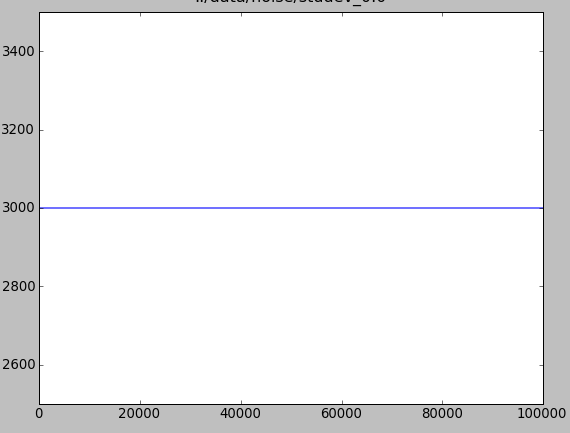
\includegraphics[width=0.22\textwidth]{figures/noise0.png}
  \label{fig:noise0}
}
\hfill
\subfigure {
  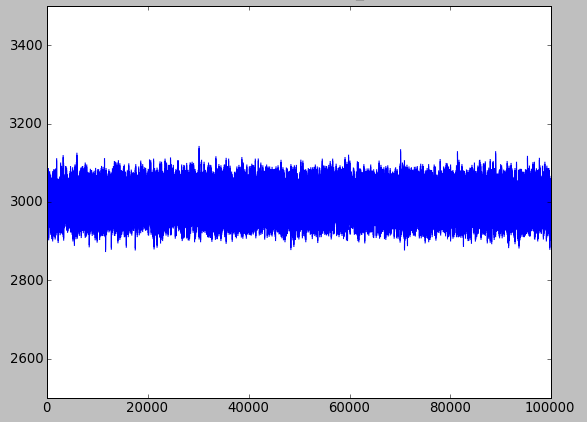
\includegraphics[width=0.22\textwidth]{figures/noise30.png}
  \label{fig:noise30}
}
\hfill
\subfigure {
  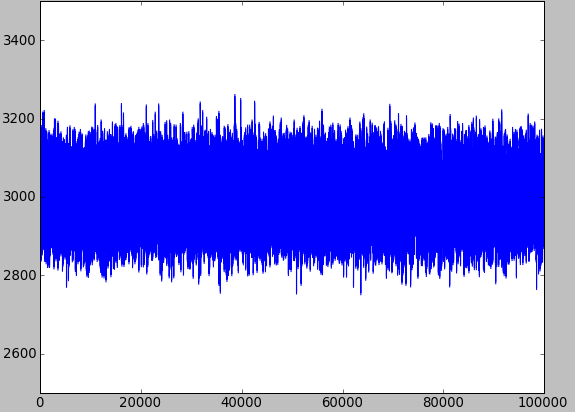
\includegraphics[width=0.22\textwidth]{figures/noise60.png}
  \label{fig:noise60}
}
\hfill
\subfigure {
  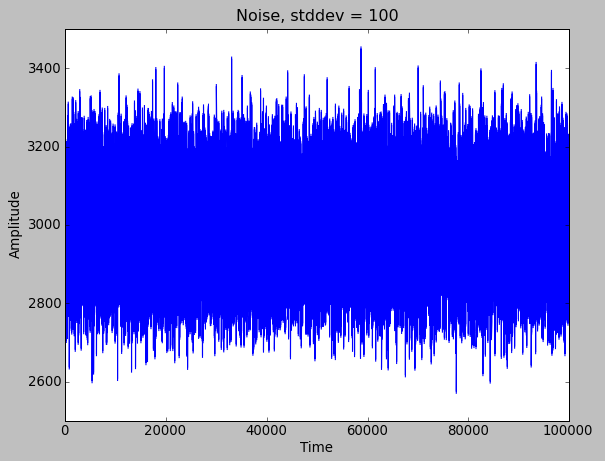
\includegraphics[width=0.22\textwidth]{figures/noise100.png}
  \label{fig:noise100}
}
\caption{Noise data set with standard deviation of 0, 30, 60 and 100}
\label{fig:noiseset}
\end{figure*}  

\begin{figure}
  \centering
  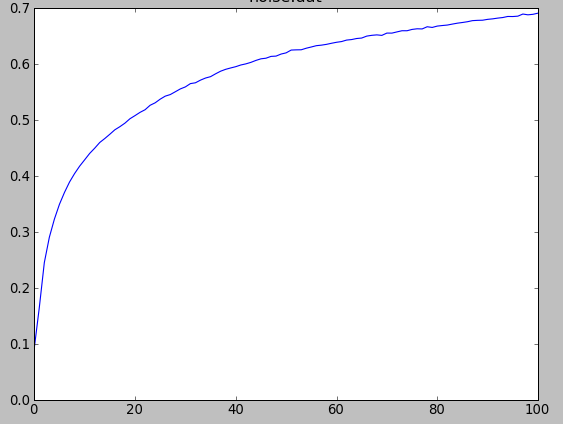
\includegraphics[width=0.50\textwidth]{figures/noiseall.png} 
  \caption{Compression ratio vs. standard deviation of noise}
  \label{fig:noiseall}
\end{figure}

\subsubsection{Energy}
